\section{Antenna Design}
\label{sec:antennadesign}
%Eventuelt noget om antenna placering i forhold til correlation
The geometry of the proposed antenna system is shown in Fig.~\ref{fig:antdesign}. The system consists of two dual-arm non-resonant antennas. The ground plane is chosen to be \SI{55}{mm} $\times$ \SI{120}{mm} which is consistent with current smartphones. For the PCB itself, a \SI{1.6}{mm} thick FR-4 substrate is used with a relative permittivity of \SI{4.4}{F/m}  and a conductivity of \SI{0.02}{S/m}. The antennas have the dimensions $7 \times 60.5 \times 5\,  \si{mm^3} \approx 2.2\,  \si{cm^3} $ 
and $7 \times 59 \times 5\,  \si{mm^3} \approx 2.1\,  \si{cm^3}$  for the top and side antenna respectively. These volumes are including the \SI{2.5}{mm} ground clearance used. The off-ground approach is used to increase bandwidth and efficiency at the lower frequency bands. Both antennas are fed through a matching circuit, consisting of three lumped elements. The matching is done with a capacitor in series followed by a shunt inductor. Lastly, a tunable MEMS  shunt capacitor is added to enable frequency reconfigurability. The MEMS tunable capacitor used is a WiSpry WS1040, which has four independent tunable capacitor-banks. Two of the banks are used for the top antenna, allowing a capacity range of \SI{0.6}{pF} to \SI{6}{pF}. For the side antenna, all four banks are used, yielding a range of \SI{1.2}{pF} to \SI{12}{pF}.

\begin{figure}[t]
  \begin{center}
    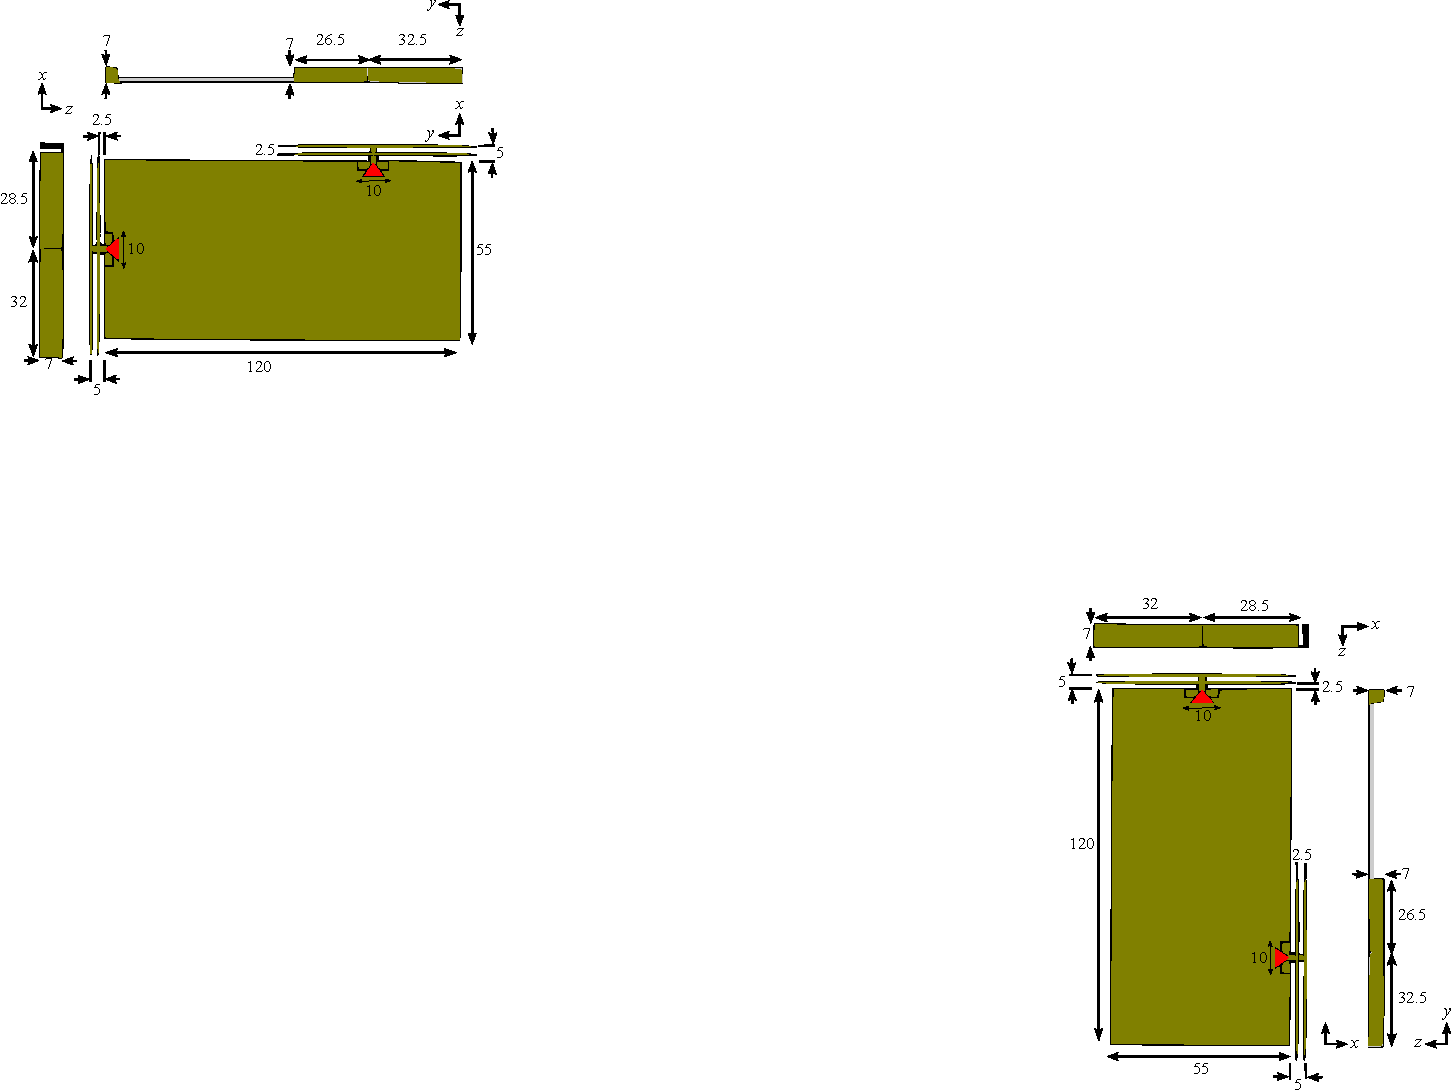
\includegraphics{img/3d_drawing}
  \end{center}
  \caption{Geometry of the MIMO antenna system.}
  \label{fig:antdesign}
\end{figure}

